% =========================
% sections/scoring_model.tex
% Operationalizing U-T-I-O as a scored index (addresses reviewer request for
% measured variables, weights, and a 0-1 scoring equation).
% =========================

\subsection{From Framework to Index: Operationalizing U-T-I-O}

The U-T-I-O Model is presented at two levels. As a \textit{descriptive framework},
it identifies the four determinant domains and their constituent constructs
(Table~\ref{tab:determinant-matrix}). As an \textit{evaluative instrument}, it can
be operationalized into a bounded alignment score for a given implementation. This
subsection specifies that operationalization so the model can be used
diagnostically, not only descriptively.

\paragraph{Measured variables.} Each domain is assessed against the construct-level
indicators defined in the scoring rubric (Supplementary File~S3), which specify
observable, evidence-anchored criteria for each domain (for example, within User
Readiness: documented usability scores, clinician-satisfaction survey results, and
patient-portal adoption rates; within Technical Interoperability: conformance to
FHIR/HL7 standards, presence of a national data-exchange layer, and semantic
mapping coverage). Each domain is rated on an ordinal four-band scale---High,
Medium, Low--Medium, Low---and mapped to a numeric domain score $d \in \{1,\,
\tfrac{2}{3},\, \tfrac{1}{3},\, 0\}$ respectively, so that each domain score lies
on the unit interval.

\paragraph{Scoring equation.} For an implementation with domain scores
$s_U, s_T, s_I, s_O \in [0,1]$ and domain weights $w_U, w_T, w_I, w_O$ with
$\sum w = 1$, the U-T-I-O Alignment Index (UAI) is the weighted mean

\begin{equation}
\mathrm{UAI} = w_U s_U + w_T s_T + w_I s_I + w_O s_O, \qquad \mathrm{UAI} \in [0,1],
\label{eq:uai}
\end{equation}

where $\mathrm{UAI}=1$ denotes full alignment across all four domains and
$\mathrm{UAI}=0$ denotes alignment absent in every domain. We report UAI under two
weighting schemes. The \textit{equal-weight} scheme ($w_U=w_T=w_I=w_O=0.25$) is
theory-neutral and makes no claim that domains differ in importance. The
\textit{evidence-weighted} scheme sets each weight in proportion to the prevalence
with which that domain is presented as an adoption determinant across the
501-study systematic evidence base (User $=0.240$, Technical $=0.247$,
Institutional $=0.234$, Organizational $=0.279$); this grounds the weights in the
observed literature rather than in author judgment. Because a compensatory
weighted mean can mask a single disqualifying deficit, we additionally report the
minimum domain score $\min(s_U,s_T,s_I,s_O)$ as a non-compensatory floor: an
implementation strong on three domains but critically weak on the fourth is
flagged by a low floor even when its UAI is moderate.

\paragraph{Worked application to the multi-case set.} Table~\ref{tab:uai} applies
Equation~\ref{eq:uai} to the national implementations. The two weighting schemes
produce near-identical orderings (Figure~\ref{fig:uai}), indicating that the
ranking is driven by the domain ratings rather than by the choice of weights.
Estonia scores at the ceiling ($\mathrm{UAI}=1.00$); ONC HIE and NHS Shared Care
Records fall in a moderate-high band ($0.83$), reflecting strong technical and
institutional alignment tempered by mixed user readiness and organizational
uptake; and the U.S. federal EHR modernization programs fall lowest. Critically,
scoring the VA and DoD programs \textit{separately}---rather than as a single
row---reveals divergence that a combined rating obscures: the VA program
($\mathrm{UAI}=0.49$, ``mixed / constrained,'' minimum domain score $\tfrac{1}{3}$)
scores materially below DoD MHS GENESIS ($\mathrm{UAI}=0.66$, ``moderate-high''),
consistent with the two programs' distinct deployment trajectories and documented
outcomes despite their shared Oracle Health (Cerner) platform. This separation is
adopted throughout the revised analysis.

\begin{table}[H]
\caption{U-T-I-O Alignment Index (UAI) for the national implementation cases}
\label{tab:uai}
\centering
\small
\renewcommand{\arraystretch}{1.3}
\setlength{\tabcolsep}{7pt}
\begin{tabular}{p{4.6cm} >{\centering\arraybackslash}p{1.1cm} >{\centering\arraybackslash}p{1.1cm} >{\centering\arraybackslash}p{1.1cm} >{\centering\arraybackslash}p{1.1cm} >{\centering\arraybackslash}p{1.6cm} >{\centering\arraybackslash}p{1.6cm} p{2.8cm}}
\toprule
\rowcolor{headerblue}
\textcolor{white}{\textbf{Case}} &
\textcolor{white}{\textbf{$s_U$}} & \textcolor{white}{\textbf{$s_T$}} &
\textcolor{white}{\textbf{$s_I$}} & \textcolor{white}{\textbf{$s_O$}} &
\textcolor{white}{\textbf{UAI (equal)}} & \textcolor{white}{\textbf{UAI (evid.)}} &
\textcolor{white}{\textbf{Interpretation}} \\
\midrule
Estonia eHealth & 1.00 & 1.00 & 1.00 & 1.00 & 1.00 & 1.00 & High alignment \\
\rowcolor{rowgray}
ONC HIE (U.S.) & 0.67 & 1.00 & 1.00 & 0.67 & 0.83 & 0.83 & Moderate-high \\
NHS Shared Care Records (UK) & 0.67 & 1.00 & 1.00 & 0.67 & 0.83 & 0.83 & Moderate-high \\
\rowcolor{rowgray}
DoD MHS GENESIS & 0.67 & 0.33 & 1.00 & 0.67 & 0.67 & 0.66 & Moderate-high \\
VA EHR (Oracle/Cerner) & 0.33 & 0.33 & 1.00 & 0.33 & 0.50 & 0.49 & Mixed / constrained \\
\bottomrule
\end{tabular}
\vspace{3pt}\\
{\footnotesize \textit{Domain scores $s$ map the four-band ordinal ratings
(High/Medium/Low--Medium/Low) to $\{1, \tfrac{2}{3}, \tfrac{1}{3}, 0\}$.
UAI is computed via Equation~\ref{eq:uai}. Evidence weights are $w_U=0.240$,
$w_T=0.247$, $w_I=0.234$, $w_O=0.279$, from 501-study domain prevalence. The VA and
DoD programs are scored separately.}}
\end{table}

\begin{figure}[H]
\centering
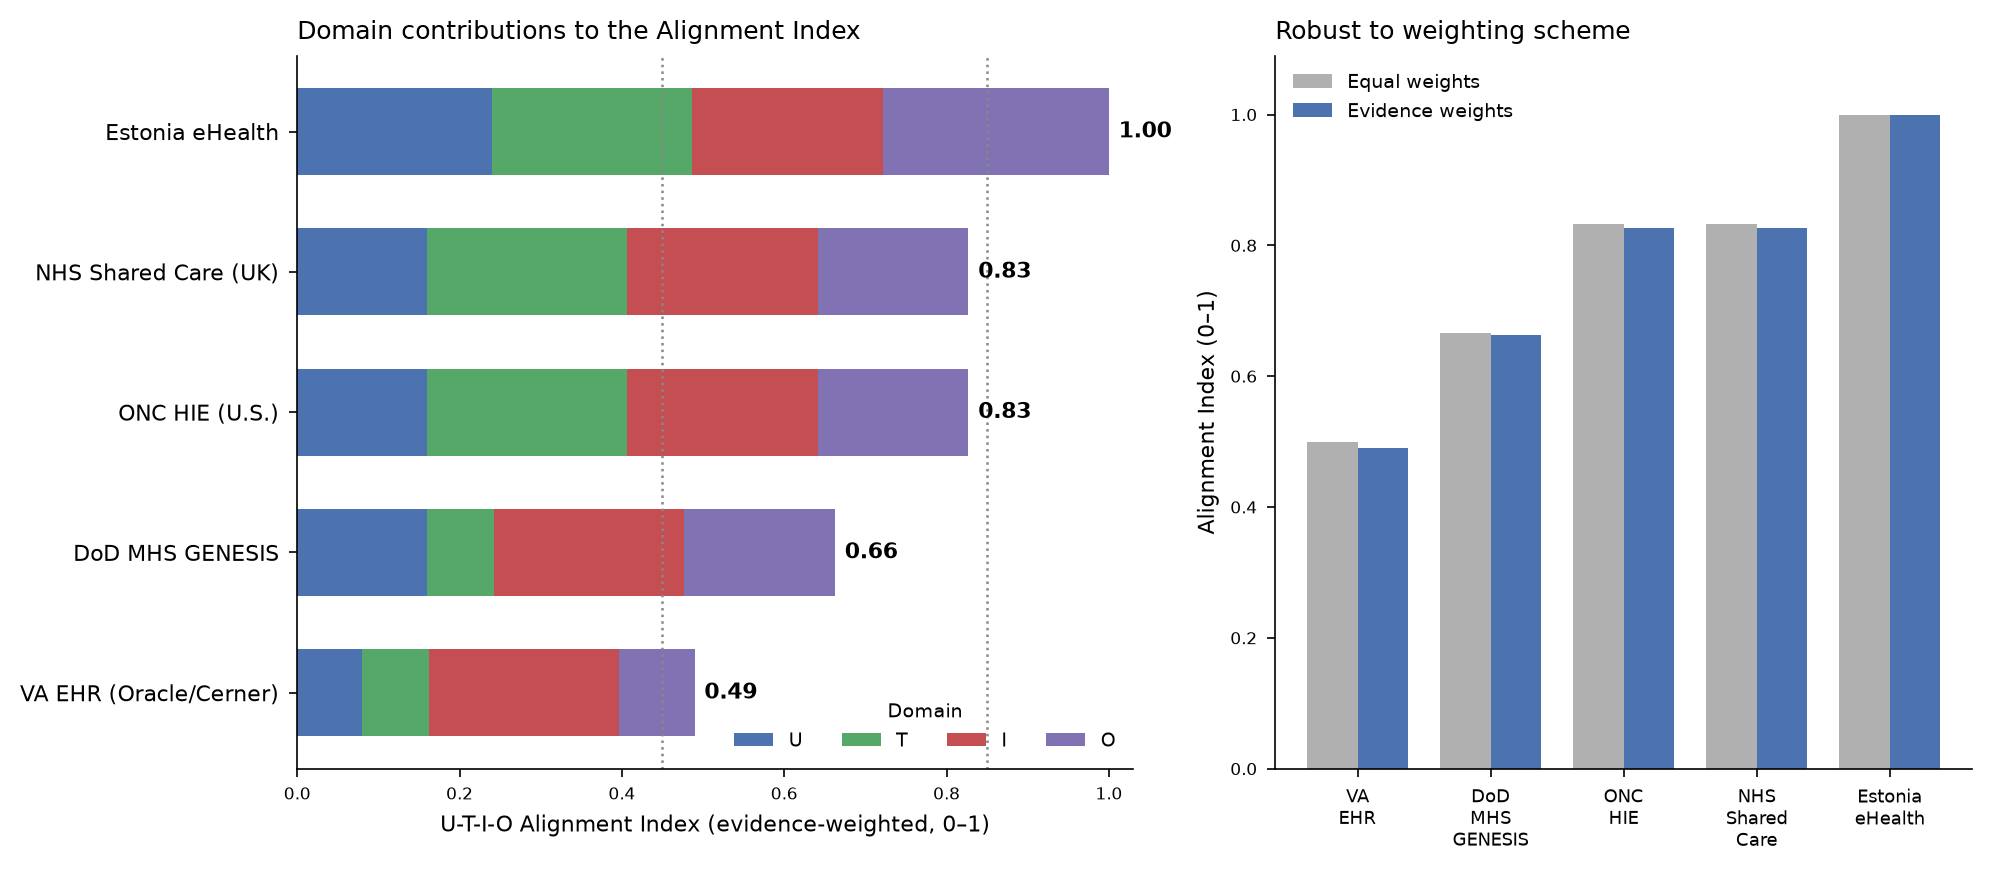
\includegraphics[width=\linewidth]{figures/utio_alignment_index.png}
\caption[U-T-I-O Alignment Index across the national cases]{U-T-I-O Alignment Index
across the national implementation cases. Left: domain contributions ($w_d s_d$)
stacked to the total index; dotted lines mark the high-alignment ($0.85$) and
mixed/constrained ($0.45$) band boundaries. Right: the index under equal versus
evidence-informed weights, showing that the ordering is robust to the weighting
scheme. Scoring the VA and DoD programs separately distinguishes VA
($\mathrm{UAI}=0.49$) from DoD MHS GENESIS ($0.66$).}
\label{fig:uai}
\end{figure}

\paragraph{Interpretation and scope of the index.} The UAI is a
\textit{readiness and diagnostic} instrument, not a validated predictive score:
it summarizes how completely an implementation aligns with the four evidence-based
determinant domains, and its non-compensatory floor localizes which domain most
constrains adoption. It is not claimed to predict clinical outcomes, which would
require the prospective outcome-linked validation described in the Limitations.
The scoring procedure is fully specified (Equation~\ref{eq:uai}, Supplementary
File~S3) so that other implementations can be scored reproducibly.
